% =====================================================================
%  IN6049 --- Forecasting and Regression Analysis
%  Week 7: Diagnostics, Remedial Measures and Nonlinear Models --- Tips dataset
%
%  Built from template/slides-template.tex (Boadilla + seahorse, 16:9).
%  Title slide + 3 recap slides + 6 week-7 slides.  Numbers come from Assigment_7.ipynb;
%  figures are its exported PNGs (images/ -> fig_*.png here).
%
%  Compiles on Overleaf with the default pdfLaTeX engine.
%  Upload alongside: fig_bands.png , fig_stab.png , fig_smoker.png ,
%  fig_deleted_residuals.png ,
%  fig_influence_map.png , fig_wls_residuals.png , fig_ridge_trace.png ,
%  fig_lowess_tree.png
% =====================================================================
\documentclass[aspectratio=169,11pt]{beamer}

\usetheme{Boadilla}
\usecolortheme{seahorse}
\setbeamertemplate{navigation symbols}{}

\usepackage[utf8]{inputenc}
\usepackage[T1]{fontenc}
\usepackage{booktabs}
\usepackage{amsmath}
\usepackage{graphicx}
\usepackage{url}

% Emphasis lead-in: bold + structure colour.  Use as \key{Finding.} text...
\newcommand{\key}[1]{\textbf{\structure{#1}}}

% Figure placeholder, so the template compiles with no image files.
% Replace each use by  \includegraphics[width=0.9\linewidth]{@@ file @@}
% (vector PDF preferred; PNG is fine).
\newcommand{\figbox}[2]{%
  \fbox{\parbox[c][#2][c]{#1}{\centering\scriptsize\color{gray}@@ figure @@}}}

% ---------------------------------------------------------------------
\title[Diagnostics and remedies]{Diagnostics, Remedial Measures and Nonlinear Models --- Tips}
\subtitle{Is the fitted model trustworthy, and what do we do when it is not?}
\author[Jie Dong, Elivier Reyes]{Jie Dong, Elivier Reyes}
\date[IN6049]{}

\begin{document}

% ===================== TITLE ========================================
\begin{frame}
  \titlepage
  \vspace{-1.2em}
  \begin{center}
    \small\urlstyle{same}\url{https://github.com/HelloJJJie/Assignment-Forecast-and-Analysis-of-Regression.git}

    \vspace{1.2em}
    The week-6 model $\hat Y=b_0+b_1\,\mathrm{bill}+b_2\,\mathrm{smoker}+b_3\,\mathrm{bill}\!\times\!\mathrm{smoker}$
    on $n=244$ bills: which cases drive it, and which remedy fits which problem?
  \end{center}
\end{frame}

% ===================== RECAP 1: SIMPLE REGRESSION ===================
\begin{frame}{Recap 1. Simple regression and inference (weeks 1--3)}
  \begin{columns}[T]
  \begin{column}{0.52\textwidth}
    \small
    \key{Model.} $\hat Y=0.920+0.105\,X$ ($X=$ bill, $Y=$ tip, $n=244$).

    \vspace{0.3em}
    {\scriptsize
    \begin{tabular}{@{}lr@{\hskip 1.2em}lr@{}}
      \toprule
      $b_1$      & $0.1050$ & $R^2$    & $0.457$ \\
      $s\{b_1\}$ & $0.0074$ & $r$      & $0.676$ \\
      $95\%$ CI  & $[0.0905,\,0.1195]$ & $s$ & $1.02$ \\
      $t^{*}$    & $14.26$  & $F^{*}$  & $203.4$ \\
      \bottomrule
    \end{tabular}}

    \vspace{0.3em}
    \begin{itemize}
      \item \key{Diagnostics:} constant variance rejected (Breusch--Pagan
            $P=4\times10^{-21}$); normality rejected ($r=0.982$ vs.\ $0.994$);
            $5$ cases with $|e^{*}|>3$.
      \item \key{Simultaneous inference:} a family $95\%$ interval for
            $\beta_0,\beta_1$ needs multiplier $2.255$ (Bonferroni), not $1.970$.
    \end{itemize}
  \end{column}
  \begin{column}{0.48\textwidth}
    \centering
    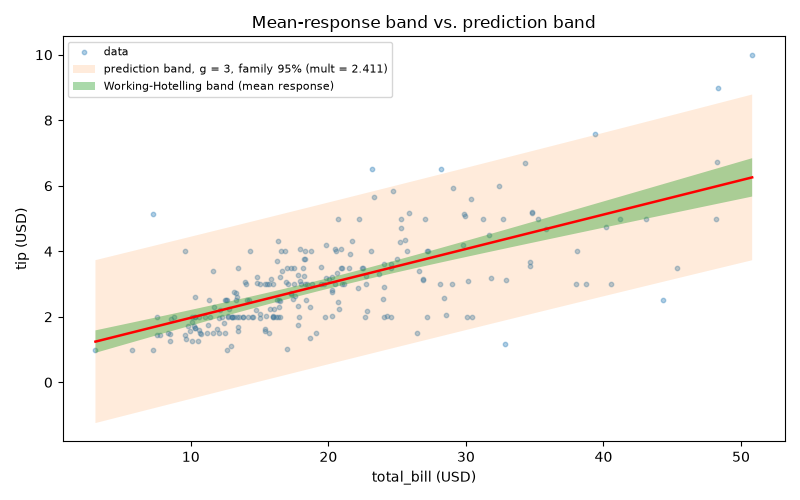
\includegraphics[width=0.84\linewidth]{fig_bands.png}

    \vspace{-0.1em}
    {\scriptsize The prediction band for new tips is about $15\times$ wider
     than the Working--Hotelling band at $\bar X$.}
  \end{column}
  \end{columns}
\end{frame}

% ===================== RECAP 2: MULTIPLE REGRESSION =================
\begin{frame}{Recap 2. Multiple regression and partial tests (weeks 4--5)}
  \begin{columns}[T]
  \begin{column}{0.52\textwidth}
    \small
    \key{Two predictors} ($X_2=$ party size): $\hat Y=0.669+0.0927X_1+0.1926X_2$,
    $F^{*}=105.95$, $R^2=0.468$ --- only $0.011$ above the bill alone.

    \vspace{0.3em}
    \begin{itemize}
      \item \key{Hat matrix:} $\mathbf H$ symmetric, idempotent, $\operatorname{tr}\mathbf H=p$;
            leverage $h_{ii}>2p/n$ for $22$ of $244$ cases.
      \item \key{Extra sums of squares depend on order:} $SSR(X_2\mid X_1)=5.2$ but
            $SSR(X_2\mid X_3)=145.3$ ($X_3=$ bill per person).
      \item \key{Multicollinearity:} adding $X_3=X_1/X_2$: $VIF=17.3,\,10.4,\,11.4$,
            the size coefficient flips from $+0.193$ to $-0.036$, $R^2$ barely moves ($0.468\to0.471$).
    \end{itemize}
  \end{column}
  \begin{column}{0.48\textwidth}
    \centering
    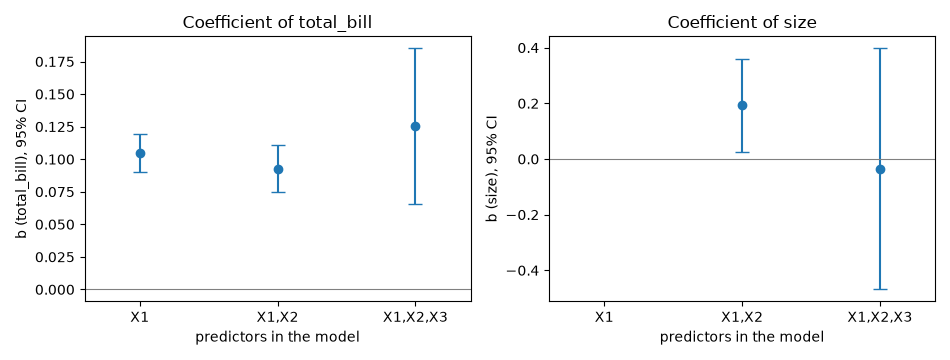
\includegraphics[width=0.96\linewidth]{fig_stab.png}

    \vspace{-0.1em}
    {\scriptsize Coefficients of bill and size as predictors enter: unstable and imprecise.}
  \end{column}
  \end{columns}
\end{frame}

% ===================== RECAP 3: INDICATORS AND SELECTION ============
\begin{frame}{Recap 3. Indicators, interaction and model selection (weeks 5--6)}
  \begin{columns}[T]
  \begin{column}{0.52\textwidth}
    \small
    \begin{itemize}
      \item \key{Qualitative predictors:} $c-1$ indicators for $c$ classes. Only
            \emph{smoker} changes the line: slope of the bill $0.137$
            (non-smokers) vs.\ $0.070$ (smokers); equal slopes rejected
            ($F^{*}=22.7$).
      \item \key{Selection:} $7$ candidates, all $2^7=128$ subsets. $R^2_a$, $C_p$, $AIC$,
            $SBC$ and $PRESS$ all pick \{bill, smoker, bill$\times$smoker\}
            ($p=4$); three stepwise paths agree.
      \item \key{Validation:} mean MSPR over $1000$ splits $1.034$ for the selected model vs.\
            $1.084$ (bill only) and $1.080$ (all seven).
      \item \key{Left open:} variance and normality still fail
            (Breusch--Pagan $\chi^2=102.6$) --- this week's starting point.
    \end{itemize}
  \end{column}
  \begin{column}{0.48\textwidth}
    \centering
    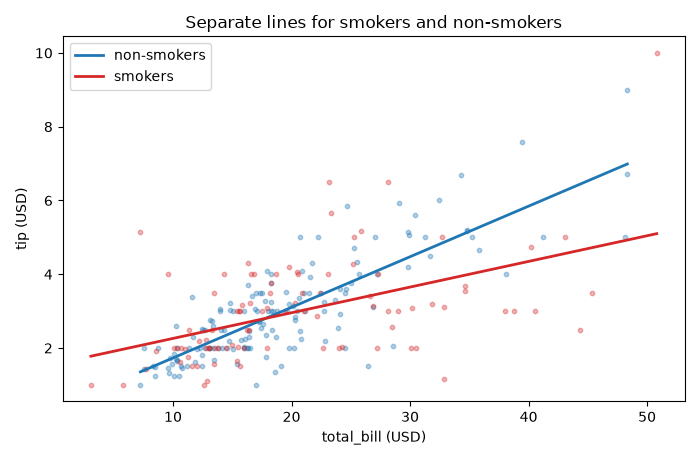
\includegraphics[width=0.92\linewidth]{fig_smoker.png}

    \vspace{-0.1em}
    {\scriptsize The model examined this week: one line per smoking status.}
  \end{column}
  \end{columns}
\end{frame}

% ===================== 1. DIAGNOSTIC MAP ============================
\begin{frame}{1. Which tool for which question: results on the selected model}
  \small
  $p=4$, $n=244$. Cut-offs as in the lecture (L7.1, slide 20):

  \vspace{0.2em}
  {\scriptsize\setlength{\tabcolsep}{3pt}
  \begin{tabular}{@{}lllp{4.9cm}@{}}
    \toprule
    Question & Tool & Flag & Result \\
    \midrule
    Right form of $X_k$?  & added-variable plot & curved / flat band & bill linear; others bend only at the ends \\
    Outlying in $Y$?      & $t_i$ (Bonferroni)  & $|t_i|>3.77$       & row $170$: $t=5.65$ \\
    Outlying in $X$?      & leverage $h_{ii}$   & $h_{ii}>2p/n=0.0328$ & $17$ of $244$ cases \\
    Influence, own fit?   & $DFFITS_i$          & $|\cdot|>2\sqrt{p/n}=0.256$ & $20$ cases; $|\cdot|>1$: row $170$ \\
    Influence, all fits?  & Cook's $D_i$        & $>F(0.50;4,240)=0.84$ & row $170$: $D=0.893$ \\
    Influence, one $b_k$? & $DFBETAS_{k(i)}$    & $|\cdot|>2/\sqrt n=0.128$ & $7$--$18$ cases per $b_k$; $|\cdot|>1$: row $170$ \\
    Redundant predictors? & $VIF_k$             & $>10$              & $1.9,\ 5.9,\ 7.1$ \\
    \bottomrule
  \end{tabular}}

  \vspace{0.4em}
  \small
  One case does most of the talking: row $170$ (0-based index; bill \$50.81, a smoker,
  tip \$10) is flagged by every tool except the form check and VIF.
  The slope of each added-variable plot equals $b_k$ (checked). VIF: only the bill is
  centered ($1.9,\,1.0,\,1.9$; centering both gives $1.04,\,1.01,\,1.03$).
  The lecture labels its DFFITS and DFBETAS cut-offs small/medium-sample;
  counts with the alternative cut-off $1$ are also reported.
\end{frame}

% ===================== 2. OUTLYING Y AND LEVERAGE ===================
\begin{frame}{2. Outlying $Y$ and outlying $X$}
  \begin{columns}[T]
  \begin{column}{0.52\textwidth}
    \small
    \key{Studentized deleted residual} $t_i\sim t(n-p-1)$; Bonferroni limit
    $t(1-\tfrac{\alpha}{2n};239)=3.77$:

    \vspace{0.2em}
    {\scriptsize
    \begin{tabular}{@{}rrrrrr@{}}
      \toprule
      row & bill & smoker & tip & $t_i$ & Bonf.\ $P$ \\
      \midrule
      $170$ & $50.81$ & $1$ & $10.00$ & $5.65$ & $<0.001$ \\
      $183$ & $23.17$ & $1$ & $6.50$  & $3.49$ & $0.14$ \\
      $172$ & $7.25$  & $1$ & $5.15$  & $3.26$ & $0.31$ \\
      \bottomrule
    \end{tabular}}

    \vspace{0.3em}
    Only row $170$ exceeds the limit; $12$ cases pass the unadjusted $1.97$,
    about the $12$ expected by chance.

    \vspace{0.4em}
    \key{Leverage:} $\bar h=p/n=0.0164$; $h_{ii}>2p/n=0.0328$ for $17$ cases
    ($10$ smokers, $7$ non-smokers), all with large bills; largest
    $0.112$ (row $170$).
  \end{column}
  \begin{column}{0.48\textwidth}
    \centering
    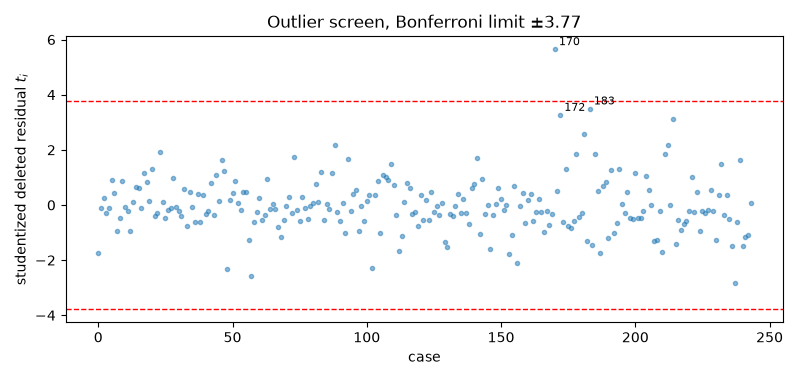
\includegraphics[width=0.90\linewidth]{fig_deleted_residuals.png}

    \vspace{0.3em}
    \raggedright\small
    \key{Hidden extrapolation:} $h_{new}=\mathbf X_{new}'(\mathbf X'\mathbf X)^{-1}\mathbf X_{new}$.
    In the week-4 model (bill, size) the point (bill $50$, size $1$) has
    $h_{new}=0.138>\max h_{ii}=0.071$ although $50$ and $1$ are each in range.
    In the selected model bill $50$ is inside ($0.0995$, $0.1069$).\par
  \end{column}
  \end{columns}
\end{frame}

% ===================== 5. INFLUENCE =================================
\begin{frame}{3. Influence: DFFITS, Cook's $D$, DFBETAS}
  \begin{columns}[T]
  \begin{column}{0.48\textwidth}
    \centering
    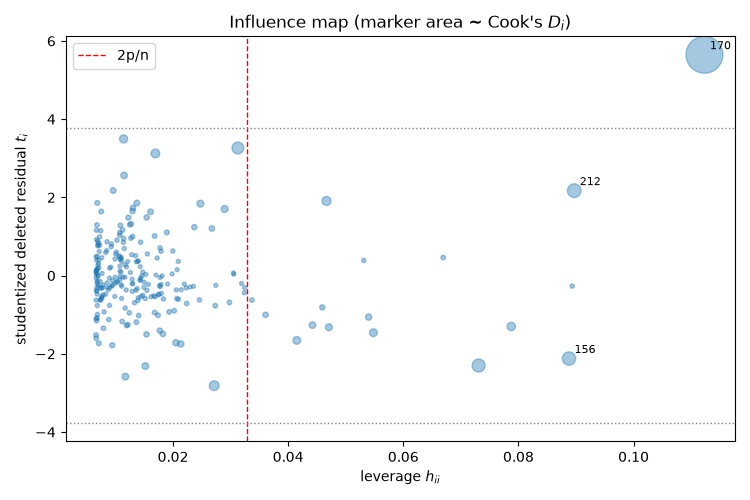
\includegraphics[width=0.94\linewidth]{fig_influence_map.png}

    \vspace{0.2em}
    {\scriptsize
    \begin{tabular}{@{}lrrr@{}}
      \toprule
       & $b_2$ smoker & $b_3$ & slope, smokers \\
      \midrule
      all cases  & $1.204$ & $-0.0676$ & $0.0696$ \\
      drop $170$ & $1.532$ & $-0.0862$ & $0.0509$ \\
      \bottomrule
    \end{tabular}}
  \end{column}
  \begin{column}{0.52\textwidth}
    \small
    {\scriptsize
    \begin{tabular}{@{}rrrrr@{}}
      \toprule
      row & $D_i$ & $DFFITS$ & $DFBETAS_{b_2}$ & $DFBETAS_{b_3}$ \\
      \midrule
      $170$ & $0.893$ & $2.008$ & $-1.115$ & $+1.397$ \\
      $212$ & $0.114$ & $0.681$ & $+0.343$ & $-0.447$ \\
      $156$ & $0.108$ & $-0.662$ & $-0.333$ & $+0.434$ \\
      \bottomrule
    \end{tabular}}

    \vspace{0.4em}
    \begin{itemize}
      \item Row $170$ is the one influential case: $D=0.893$ is above the
            $50$th percentile of $F(4,240)$ ($0.84$); no other $D$ passes the $20$th ($0.41$).
      \item It moves $b_2$ and $b_3$ by more than one standard error (DFBETAS) but
            not the bill slope: it is a smoker.
      \item \key{Sensitivity:} without it the smokers' slope \emph{falls}
            ($0.070\to0.051$): the case pulled the two lines together.
    \end{itemize}
  \end{column}
  \end{columns}
\end{frame}

% ===================== 4. WLS, ROBUST, BOOTSTRAP ====================
\begin{frame}{4. Remedies: weighted, robust and bootstrap estimates}
  \begin{columns}[T]
  \begin{column}{0.56\textwidth}
    \small
    \key{Estimates.} WLS: $w_i=1/\hat s_i^{2}$, $\hat s_i$ from $|e_i|$ on $\hat Y_i$.
    Robust: M-estimation (Huber, Tukey biweight).

    \vspace{0.2em}
    {\scriptsize\setlength{\tabcolsep}{3pt}
    \begin{tabular}{@{}lrrrr@{}}
      \toprule
       & OLS & WLS & Huber & Tukey \\
      \midrule
      $b_2$ (smoker)      & $1.204$   & $1.069$   & $1.206$   & $1.289$ \\
      $b_3$ (interaction) & $-0.0676$ & $-0.0605$ & $-0.0761$ & $-0.0835$ \\
      slope, smokers      & $0.0696$  & $0.0756$  & $0.0605$  & $0.0542$ \\
      \bottomrule
    \end{tabular}}

    \vspace{0.2em}
    {\scriptsize OLS without row $170$: smokers' slope $0.0509$. Tukey weight $0$ for rows
    $170$ and $183$.}

    \vspace{0.3em}
    \small
    \key{Standard errors} (bootstrap: $B=2000$ resamples of cases):

    \vspace{0.2em}
    {\scriptsize\setlength{\tabcolsep}{3pt}
    \begin{tabular}{@{}lrrrr@{}}
      \toprule
       & OLS se & HC3 se & boot se & WLS se \\
      \midrule
      bill          & $0.0097$ & $0.0118$ & $0.0112$ & $0.0108$ \\
      smoker        & $0.312$  & $0.466$  & $0.430$  & $0.268$ \\
      bill$\times$smoker & $0.0142$ & $0.0255$ & $0.0232$ & $0.0155$ \\
      \bottomrule
    \end{tabular}}
  \end{column}
  \begin{column}{0.44\textwidth}
    \centering
    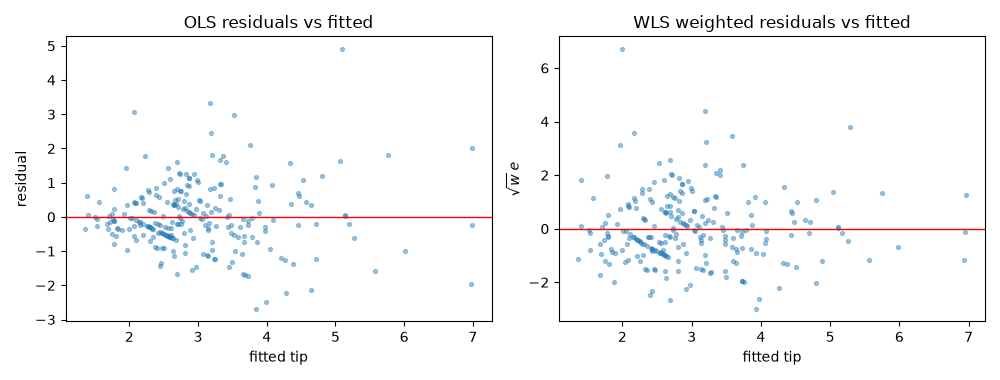
\includegraphics[width=0.98\linewidth]{fig_wls_residuals.png}

    \vspace{0.1em}
    \raggedright\scriptsize
    Residual sd by thirds of the fit: OLS $0.66/0.83/1.31$, weighted
    $1.34/1.23/1.36$. Breusch--Pagan on the weighted residuals still
    rejects ($\chi^2=28.3$ vs.\ $102.6$): the funnel is largely, not entirely, removed.

    \vspace{0.2em}
    \small
    The bootstrap agrees with HC3, not with the ordinary se: $b_3$ $95\%$ CI
    $[-0.112,\,-0.020]$ excludes $0$.\par
  \end{column}
  \end{columns}
\end{frame}

% ===================== 8. RIDGE AND NONPARAMETRIC ===================
\begin{frame}{5. Ridge regression, lowess and trees}
  \begin{columns}[T]
  \begin{column}{0.50\textwidth}
    \centering
    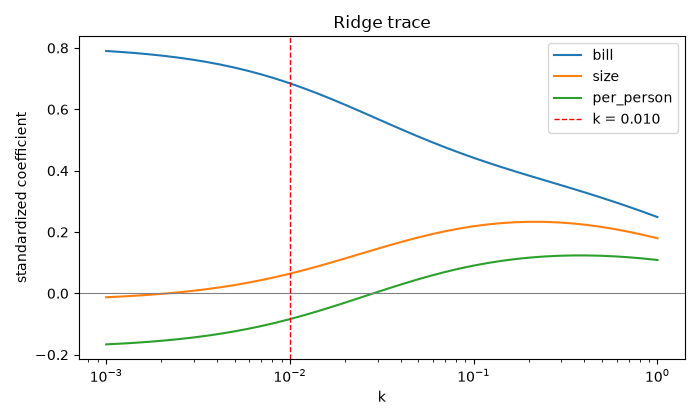
\includegraphics[width=0.92\linewidth]{fig_ridge_trace.png}

    \vspace{0.2em}
    \raggedright\scriptsize
    Ridge needs collinear predictors, so it uses the week-5 set (bill, size,
    bill per person; VIF $17.3,\,10.4,\,11.4$). $k=0.010$ is the smallest on the
    grid with every ridge VIF $<10$: $R^2$ $0.4707\to0.4698$; the size coefficient
    ($-0.024$) turns positive.\par
  \end{column}
  \begin{column}{0.50\textwidth}
    \centering
    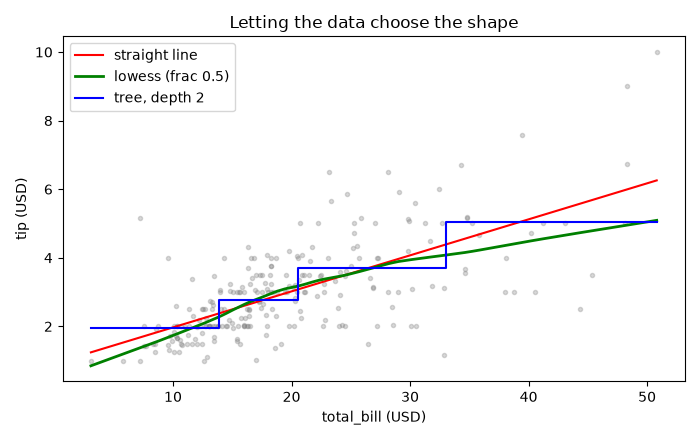
\includegraphics[width=0.92\linewidth]{fig_lowess_tree.png}

    \vspace{0.2em}
    \raggedright\scriptsize
    Lowess ($0.5$ of the data per window) and a depth-$2$ tree (splits at bill
    $13.81$, $20.45$, $32.90$) do not beat the straight line in sample: SSE
    $261.0$ and $263.4$ vs.\ $252.8$. The data show no shape the line misses.\par
  \end{column}
  \end{columns}
\end{frame}

% ===================== 9. NONLINEAR, NN, SUMMARY ====================
\begin{frame}{6. Nonlinear regression, a neural network, and the big picture}
  \begin{columns}[T]
  \begin{column}{0.46\textwidth}
    \small
    \key{Nonlinear least squares:} $\mathrm{tip}=a\cdot\mathrm{bill}^{c}$,
    $c=0.71$ ($95\%$ CI $[0.61,\,0.81]$): tips grow less than proportionally.
    SSE $253.0$ vs.\ $252.8$ for the line --- same fit, two parameters.

    \vspace{0.4em}
    \key{Neural network} (4 hidden units; bill, smoker; $100$ random $50/50$ splits):

    \vspace{0.2em}
    {\scriptsize
    \begin{tabular}{@{}lrr@{}}
      \toprule
       & train MSE & MSPR \\
      \midrule
      selected linear model & $0.890$ & $1.059$ \\
      network               & $0.667$ & $1.421$ \\
      \bottomrule
    \end{tabular}}

    \vspace{0.2em}
    \scriptsize The network overfits: better in sample, worse out of sample
    (smaller MSPR in $17\%$ of splits).\par
  \end{column}
  \begin{column}{0.54\textwidth}
    \small
    \key{Problem $\to$ remedy $\to$ what happened here}

    \vspace{0.2em}
    {\scriptsize\setlength{\tabcolsep}{3pt}
    \begin{tabular}{@{}lll@{}}
      \toprule
      Problem & Remedy & Result \\
      \midrule
      unequal variance & WLS         & flat spread; BP still rejects \\
      collinearity     & ridge       & $k=0.01$, $R^2$ $-0.001$ \\
      influential case & robust      & slope $0.070\to0.054$--$0.061$ \\
      unknown shape    & lowess/tree & no gain over the line \\
      no se formula    & bootstrap   & agrees with HC3 \\
      curved, meaningful & nonlinear & $c=0.71$, same SSE \\
      complex pattern  & network     & overfits \\
      \bottomrule
    \end{tabular}}
  \end{column}
  \end{columns}
\end{frame}


\end{document}
